\documentclass[titlepage]{article}
\usepackage{fullpage}
\usepackage{graphics,indentfirst,amsmath,amsthm,amssymb,latexsym,enumerate}
\usepackage{graphicx}
\begin{document}

\title{17-651 Models of Software Systems\\[1ex] Project 1: Nicebook}
\author{
{\Large\textbf{Group 9}}\\[3ex]
Ajay Nair\\[1ex] Huairui Qi\\[1ex] Yu-Chun Shih\\[1ex] Nianjie Wan\\[1ex]Songbo Wu}
\date{\today}
\maketitle

\section{Task 1 - Basic Social Network}

\subsection{Object Model}
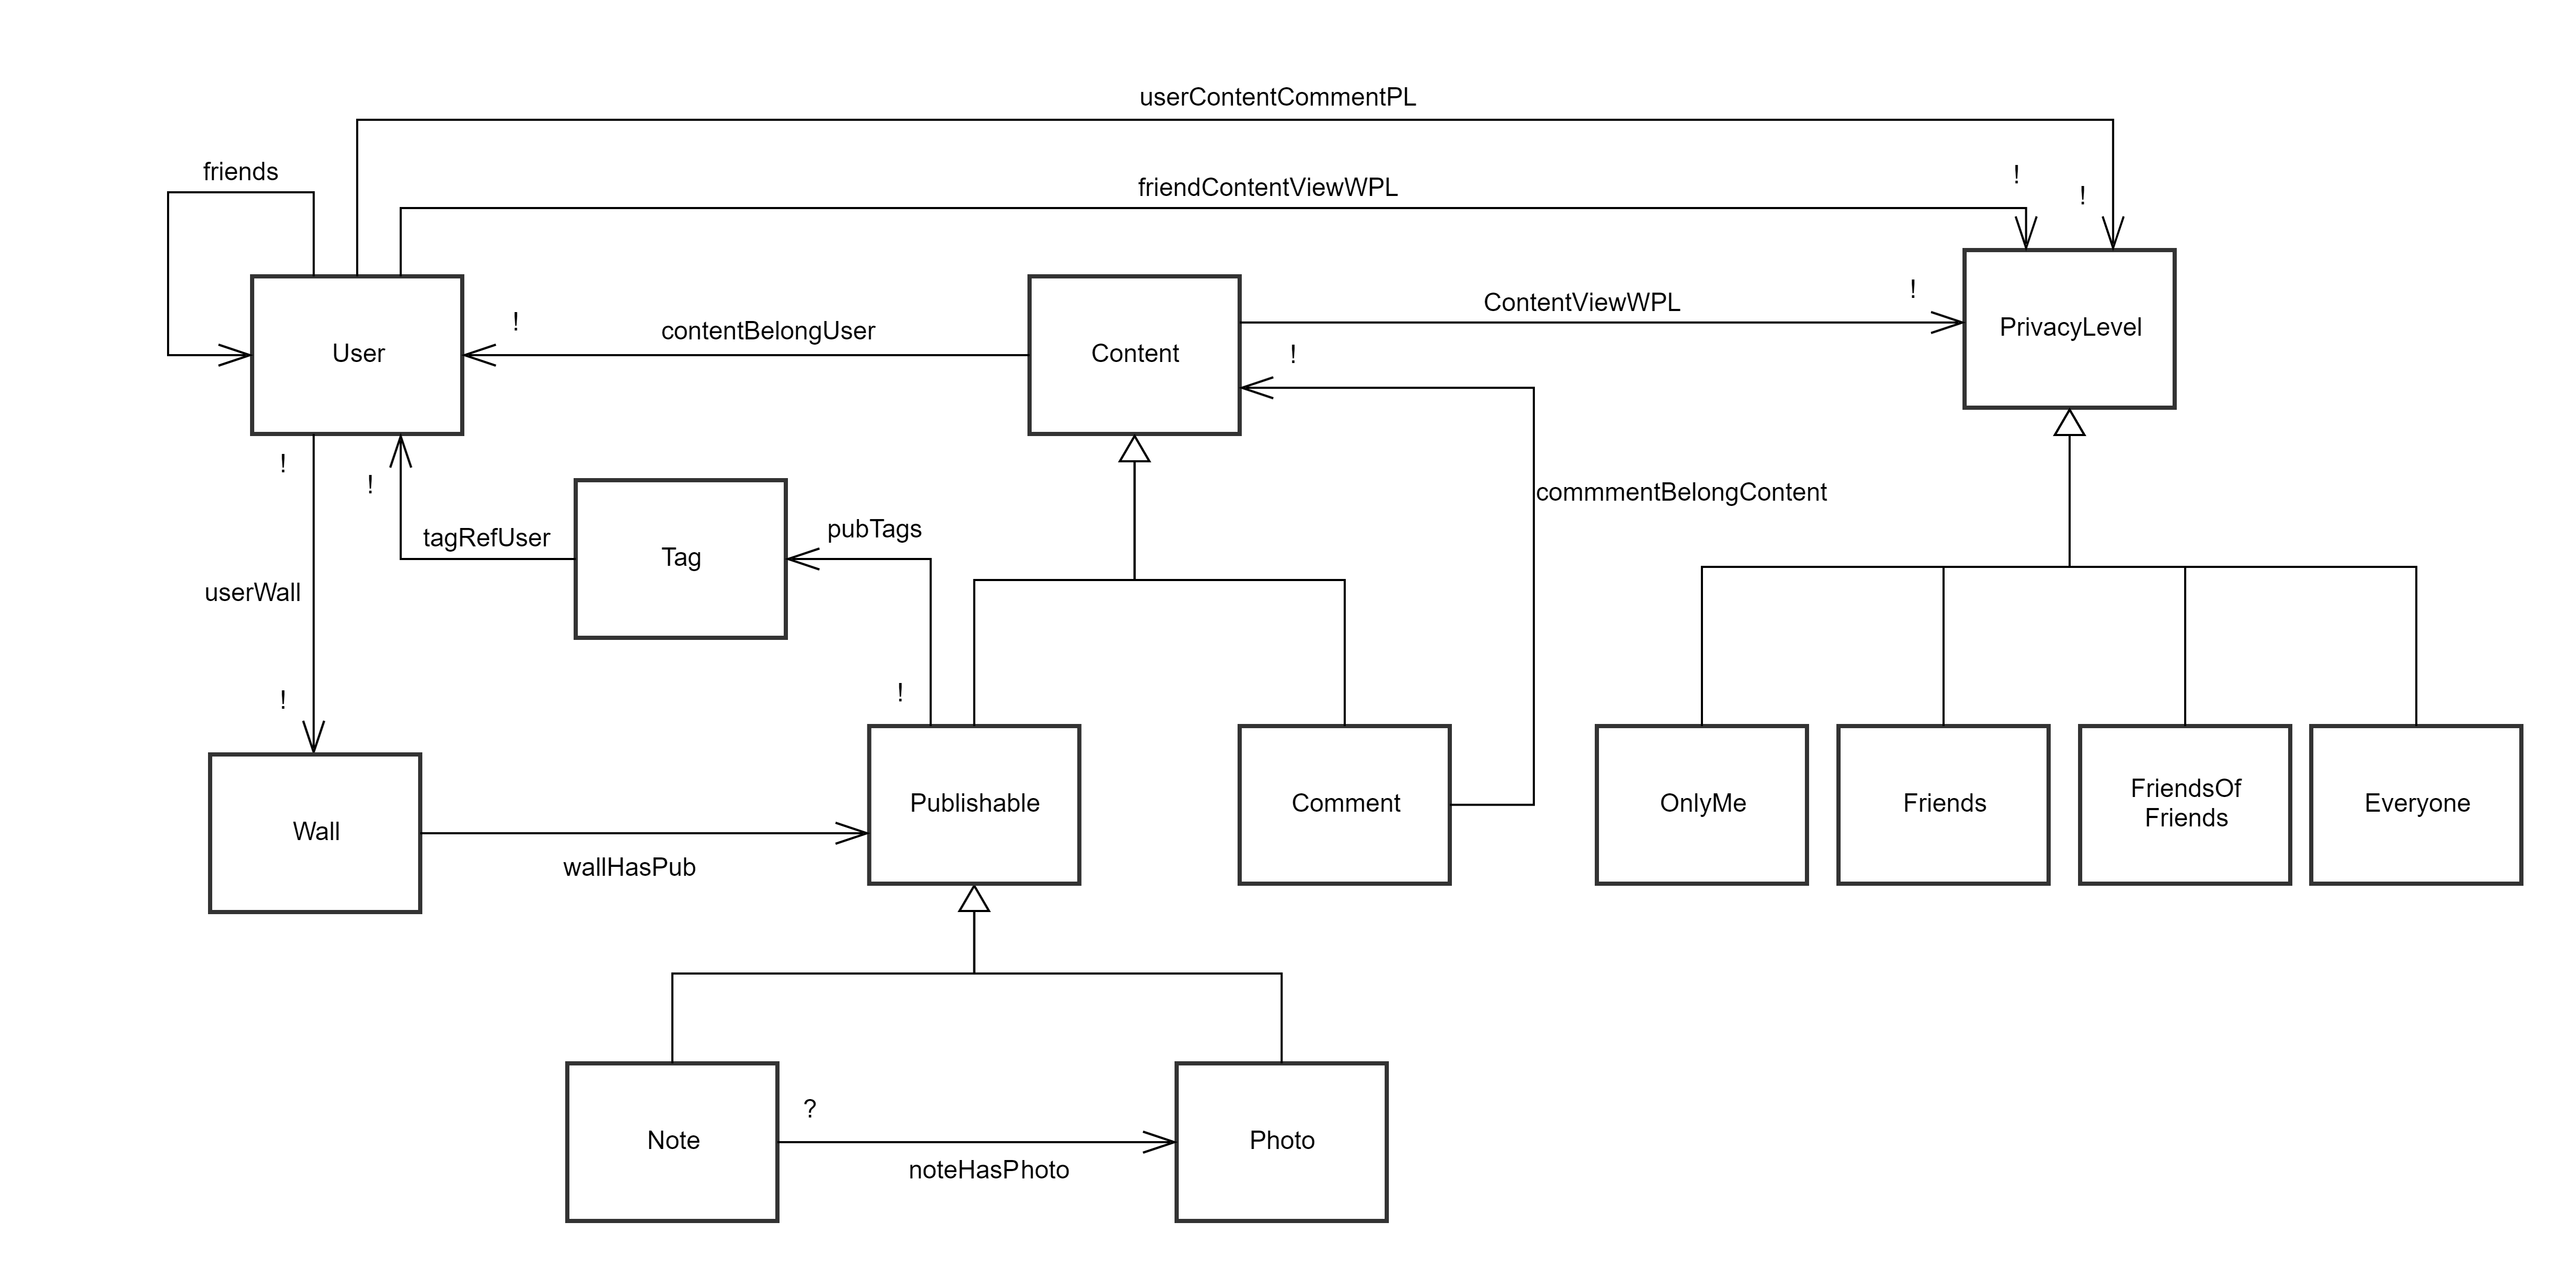
\includegraphics[width=6in]{NiceBookObjectModel.png}

The relationships between \texttt{User}, \texttt{Content} and \texttt{PrivacyLevel} - \texttt{friendContentViewWPL}, \texttt{ContentViewWPL} and \texttt{userContentCommentPL} denotes the three privacy level settings that the users and contents are associated with. The relationship between \texttt{Tag} and \texttt{User} called \texttt{tagRefUser} points to the user the tag is referencing, and the relationship between
\texttt{Tag} and \texttt{Publishable} called \texttt{pubTags} is the set of tags included in a publishable. The naming convention is that each relation-name has the name of the signature it points to as part of the relation-name. In short, if the relationship is linked from A to B, we then put the relation-name as $A[verb]B$.

Since \texttt{Content} includes \texttt{Comment}, \texttt{Note} and \texttt{Photo}, and the last two are publishable, we have two exhausted subsets - \texttt{Comment} and \texttt{Publishable} as subsets of \texttt{Content} and \texttt{Note} and \texttt{Photo} as  subsets of \texttt{Publishable}.

\subsection{Ambiguities and Decisions}
\label{Ambiguities}
During the analysis of the specification of Nicebook, we identified the following ambiguities regarding the basic definition of it.

\begin{enumerate}
    \item The spec doesn't mention anything about whether a note or a photo can be published on multiple walls at the same time.\\
    \textbf{Decision:} It can be published onto multiple walls. We come to this decision because \textit{the content in which a user is tagged is automatically published onto \textbf{that user}’s wall}. A content can certainly have multiple tags, so that it should be allowed to be published to multiple walls in order to support this requirement.
    
    \item Is it allowed for a photo to be contained in multiple notes?\\
    \textbf{Decision:} No, it's not allowed. This is because people may make irrelevant comments to the same photo in different notes as it will have different context. That is to say, even if the same photo is contained by two different note, we then consider the two instances of the photos as two unique photos because they may be attached to different streams of comments.
    
    \item The specification doesn't have any constraints for how many tags can a user have. In addition, is a tag allowed to be associated with more than one piece of content?\\
    \textbf{Decision:} One user can have multiple tags. This is because we consider that tags that reference the same user but appear in different contents are different from each other. Moreover, a tag is not allowed to be associated with more than one content, since each tag that appears on the content is unique.
    
    \item What is the meaning of \textit{publish}? If only notes and photos can be published on walls, what about comments for the published notes and photos? Are they published?\\
    \textbf{Decision:} There is a constraint in the specification that says \textit{content must be published on a wall before it can be viewed by users other than its owner}. In other words, all the contents on the wall are published. However, only notes and photos can be directly published onto a wall. Comments have to be attached to some notes or photos. In addition, a comment is said to be \textit{published} if and only if the highest root(a note or a photo) is published.
    
    \item Is it allowed for a published note to contain some photos that are not published?\\
    \textbf{Decision:} We think this is allowed. If some photos are missing from its parent note, we think it would make no sense if the users couldn't see the other photos in that note that are not missing.
    
\end{enumerate}

Furthermore, there are also several ambiguities regarding the operations:

\begin{enumerate}
    \item What does it mean to remove a note that contains other photos? Should the contained photos be automatically removed with the operation?\\
    \textbf{Decision:} No, they should not be automatically removed. We come to this decision because we think that removing a note does not necessarily means that the user wants to remove all the photos in it. Maybe it's just the note that the user wants to remove. However, once the note has been removed, the contained photos should no longer be contained by it(there should be no containment relationship anymore).

    \item What does it mean to publish/unpublish a note that contains other photos? Are the photos contained by the note published/unpublished automatically? \\
    \textbf{Decision:} We decide that the contained photos should be published/unpublished automatically because they have a containment relationship with the parent note. But this does not say that the user cannot unpublish/publish the contained photos from/onto the wall later. Please refer to the fifth item on the previous list.
    
    \item What happens to the comments of the contents that are already published on some wall but get unpublished/removed after the comments have been made?\\
    \textbf{Decision:} We think a comment should be made viewable only to its owner after the commented content is unpublished. And a comment should be removed if the comment's content is removed.
    
    \item What does it mean to unpublish a comment from a wall if a comment cannot be directly published to a wall?\\
    \textbf{Decision:} It's not allowed to unpublish or remove a comment.
    
    \item What does it mean to remove a tag? Should the content from which the tag is removed be automatically unpublished from the wall of the tagged user?\\
    \textbf{Decision:} Removing a tag means that the relationship between the publishable and the tag is no longer exist. No, it should not be automatically unpublished.
\end{enumerate}

There are some other very important design decisions we made throughout this project:

\begin{enumerate}
    \item We think it's unreasonable to upload a comment to Nicebook that is not attached to any other content because no existing application is doing that. Every comment has to come with a content that it's attached to.\\
    \textbf{Decision:} We decide that it's not allowed to \texttt{upload} comment without adding it to an existing content. Furthermore, the specification says that \textit{comments can not be deleted}. As a result, we don't have the operation of \texttt{UploadComment}. Instead, we only have \texttt{AddComment} operation.
    
    \item We think it's unreasonable to enforce that a user must have at least one piece of content because it's possible that a user has no content  but only want to view other people's contents.\\
    \textbf{Decision:} We decide that a user \textbf{may} have one or more pieces of content instead of \textbf{must}.
\end{enumerate}

\subsection{Invariant Discovered}

Some of the invariants were not discovered until we started to write the operations. Some of them are:

\begin{enumerate}
    \item If content has a tag, then it has to be published onto the wall of the user that the said tag is referencing. 
    \item The child comments privacy level should be lower or equal to the parent node privacy level. We think this is valid because a comment should be visible if all its parents are visible otherwise the user reading the comment may not get the context of the comment. 
    \item The user can unpublish content from the user's wall or content published by the user of another user's wall. We think this is valid because the user should have control over the content that the user has published. The user should also have access to their own wall.
\end{enumerate}

\subsection{An Example of Invariant Violated by Operations}

\textbf{Problem} : As mentioned in section~\ref{Ambiguities}, our team decided that a comment can only be created as a brand new content that is not uploaded yet in the user’s account, which means that the comment can only be added to an existing content already published on some user’s wall. Besides, the comment can only be added to the contents of his/her friends and himself/herself. When our team was trying to write the operation \texttt{uploadPub}, we found that some comments were attached to contents that were not in the same Nicebook instance as the said comments.

\textbf{Problem solution} : The solution our team discussed and applied to solve the problem was that - in comment signature, we define that each comment should belong to exactly one content, and then we make a constraint enforces that all the commented contents should be in the same Nicebook instance as the said comments.
      
    
\subsection{Scope of Invariant Preservation Analysis}
Scope used for invariant preservation : 5.

We used 5 as the scope for the invariant preservation analysis for every operation. Additionally, there are 4 privacy levels and so we believe the scope should be 4/5 so that we test for a combination of each content having all the privacy level.

Fortunately, counterexamples tend to appear in small-size examples, so we believe 5 would be sufficient.

\section{Task 2 - Privacy Control}
\subsection{Privacy Policy}
In this section, we introduce the privacy policy for Nicebook, which is basically how we interpret the three privacy settings described in the specification.

\begin{enumerate}
    \item Each content has a privacy setting called \texttt{contentViewWPL}, where WPL is the abbreviation for WallPrivacyLevel. This setting controls who can view a user's content on the said user's wall.
    \item Each user has a privacy setting called \texttt{friendContentViewWPL} This setting controls who can view the other users' contents on the said user's wall. In other words, if \texttt{UserA} has a \texttt{Photo} on \texttt{UserB}'s wall, then who can view \texttt{Photo} via \texttt{UserB}'s wall is controlled by \texttt{friendContentViewWPL} of \texttt{UserB} instead of by \texttt{Photo}'s {contentViewWPL}.
    \item Each user has a privacy setting called \texttt{userContentCommentPL} that controls who is able to comment on the contents of the said user.
\end{enumerate}

\subsection{\texttt{NoPrivacyViolation} Analysis}
Our model satisfies \texttt{NoPrivacyViolation}, since all of our operations have preserved the invariant which we checked using the assertion. We have implemented a function called \texttt{getGroup} which returns the group of users that a particular privacy level suggests with respect to the given user. In addition, we implemented another function called \texttt{contentViewer} to return the set of users that are available to view a piece of content based on the content's privacy level. With the help of these two functions, we are able to make sure that none of our operations violate privacy constraints. For example, in \texttt{AddComment}, we have stated in the precondition that the owner of the comment must be in the \texttt{contentViewer} set of the content the comment is attached to, also the owner of the comment must be in the set of users that the owner of the content the comment is adding on with respect to the privacy level the content owner has set. All the above privacy level constraints can be successfully preserved with the helper functions that we have designed.

In the spec of the social network, it does not mention whether users can view the child comment if the child comment has less restrictive privacy violation than its parent-content. To resolve this ambiguity, we decide to add a constraint that the privacy level of the child comment should have an equal or more restrictive privacy level than its parent. This is the alternative that we discovered and the resolution that we come up with.
\end{document}